\chapter[Visão do Produto]{Visão do Produto}

\section{Visão Estrutural}

Ao desenhar a estrutura do Robô foi identificado que deve-se levar em consideração os seguintes aspectos:
\begin{enumerate}
	\item Melhor identificação da criança com o equipamento
	\item Segurança
\end{enumerate}

Melhor identificação da criança com o equipamento:
\begin{itemize}
\item Cor: Pagnan, C. M. et al afirma que a cor exerce uma ação tríplice: a de impressionar a de expressar e a de construir, portanto o
aparelho deve apresentar coloração atrativa para a criança, e também faz uma relação entre as cores e as respectivas características
psicológicas e simbólicas, para os propósitos do trabalho selecionamos duas cores:
\item Azul: Exerce apelo intelectual, simbolizando a inteligência e raciocínio.
\item Vermelho: Estimulante e dinâmica é a cor preferida da criança.
\item Aparência: Quanto a aparência ela deve ter aparência agradável, intuitiva e associado a elementos que o usuário conheça e se
identifique, as formas especuladas são veículos e elementos de filmes desenhos e etc.
\end{itemize}

\textbf{Segurança}:
O produto oferecido não deve apresentar nenhum tipo de risco a integridade física da criança, portanto o produto deve possuir design
“macio”, não apresentando pontas ou qualquer componente que venha a amplificar um possível tipo de dano causado por contato mecânico.

\textbf{Design}:
A estrutura foi desenhada no software CATIA, o intuito foi lembrar a estrutura de um carrinho, elemento a qual a criança já está
acostumada. Alguns elementos como iluminação a led e desenhos vão ser introduzidos na estrutura física final de modo a tornar o
carrinho ainda mais atrativo para a criança.

\begin{figure}[H]
    \centering
    
\includegraphics[width=0.8\textwidth]{figuras/estrutura_catia.eps}
    \caption{}
    \label{fig:catia01}
\end{figure}

\textbf{Peso}: Ao realizar o assembly das peças no CATIA utilizou –se uma ferramenta no próprio software para estimar o peso do carrinho,
o valor obtido foi de aproximadamente 3,5 Kg. Porem como faltou o cad de alguns dos componentes o valor da massa utilizado nos demais
cálculos foi de 4 Kg para contabilizar eses componentes e oferecer uma certa margem de erro.


- \textbf{Materiais}:
Para selecionarmos o material a ser utilizado na estrutura os critérios considerados foram:
\begin{itemize}
\item Segurança
\item Propriedades mecânicas
\item Proteção dos equipamentos eletrônicos
\end{itemize}

Inicialmente foi considerado a escolha de dois tipos de materiais o alumínio e polímeros.
 
Segurança da criança: Nesse aspecto os riscos identificados foram:
\begin{enumerate}
\item Toxicidade
\item Choques mecânicos
\end{enumerate}

Segundo a Ficha de informações de segurança do produto químico da The Dow Chemical Company o HDPE não é uma Substância Química Perigosa,
classificado pela definição do Padrão OSHA de Comunicação de Perigos, 29 CFR 1910.1200. Ainda segunda a The Dow Chemical Company o contato
prolongado não é irritante para a pele e nem a pele absolve de alguma maneira o material, portanto os principais riscos que o material
deve apresentar são inerentes a todos os materiais e se devem a choques mecânicos. Esses choques mecânicos podem ser amenizados dependendo
do processo de fabricação, que pode ser escolhido para produzir um material mais ‘macio’ e que ao mesmo tempo aguente os esforços
mecânicos a qual o robô será submetido.

Propriedades mecânicas: Os principais esforços identificados a qual o robô será submetido foram:
\begin{enumerate}
\item Queda
\item Peso (devido a objetos em cima do robô)
\item Choques com obstáculos
\end{enumerate}

\begin{figure}[H]
    \centering
    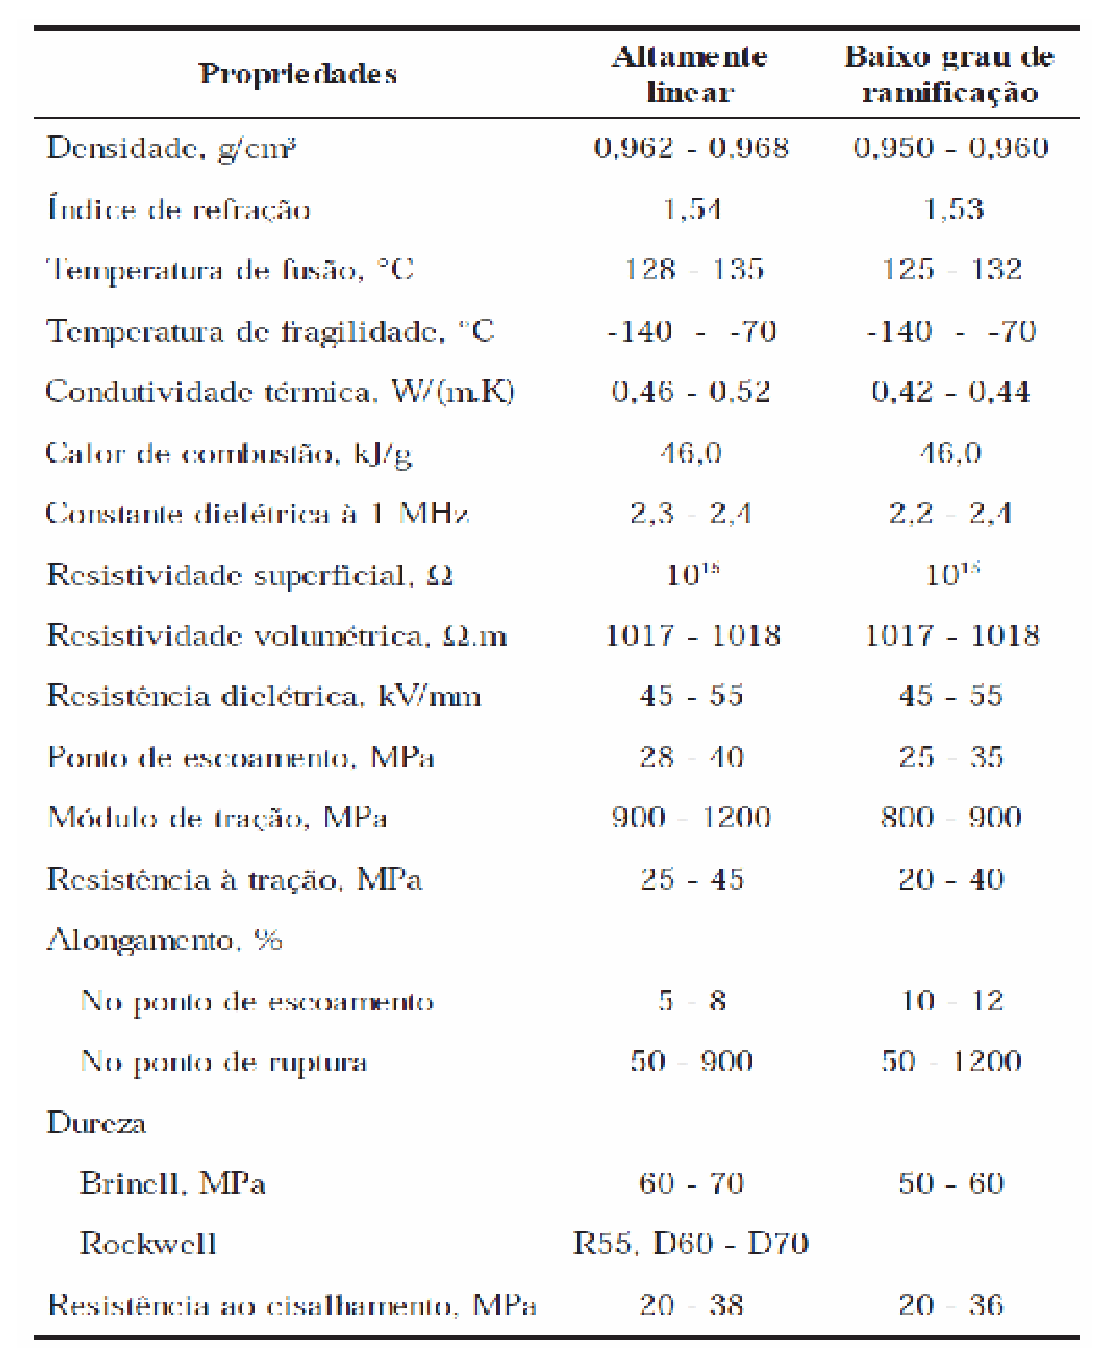
\includegraphics[width=0.4\textwidth]{figuras/tabela_pead.eps}
    \caption{Propriedades do HDPE}
    \label{fig:pead}
\end{figure}

Em comparação com o alumínio que foi o outro material considerado que é comumente usado nesse tipo de aplicação, essas propriedades
validam o uso do HDPE no projeto. O grande diferencial do HDPE foi o preço e a maior facilidade de conformar o material para forma
desejada. Segue abaixo uma tabela com as propriedades do alumínio CAST 7000, um dos mais usados para construção de chassi de maquinas no geral:

Proteção dos equipamentos eletrônicos: Nesse tópico as principais preocupações foram:
\begin{enumerate}
\item Transferência de calor.
\item Condução elétrica.
\end{enumerate}

Como podemos ver, o HDPE apresenta as propriedades de condução térmica e elétrica em ordens de grandeza bem menor que a do alumínio.
Portanto é o mais indicado nesse quesito.

De todos os 3 aspectos considerado o HDPE apresenta um maior número de vantagens em todos, no quesito das propriedades mecânicas embora
o alumínio ofereça propriedades mecânicas superiores, esses valores estão muito acima da necessidade do projeto, logo o HDPE foi o
material selecionado para desenvolvermos o chassi do robô.
 
\textbf{Analise Estrutural}

A análise estrutural foi realizada no software ASYNS e foi feita apenas para o caso estático. No caso dinâmico, o software recebe os
parâmetros físicos do carrinho e as condições de contorno que seria a de uma free wall, ao final da simulação o software retorna os
valores dos parâmetros em um intervalo de tempo. Esse tipo de simulação é muito complexa e geralmente requer grande poder de processamento.
O caso estático funciona de maneira semelhante porem as condições de contorno são diferente e o resultado é valido apenas para uma
unidade de tempo, nesse tipo de simulação deve ser feita uma análise antes de maneira a obter os resultados no tempo certo.

Os parâmetros analisados foram a deformação que a estrutura sofre, e a tensão de Von Mises que é um critério utilizado para prever a
falha de materiais frágeis.

\textbf{Queda}: no caso da queda a unidade de tempo desejada é a que a magnitude da força atuando sobre o carrinho seja a maior possível.
As condições de contorno são: um lado do carrinho sem sofrer deslocamento estrutural (deformação) e em algum outro lado aleatório
(foi testado em todos os lados) aplica-se uma força igual a força atuante na hora do impacto:

\textbf{Deformação}:

\begin{figure}[H]
    \centering
    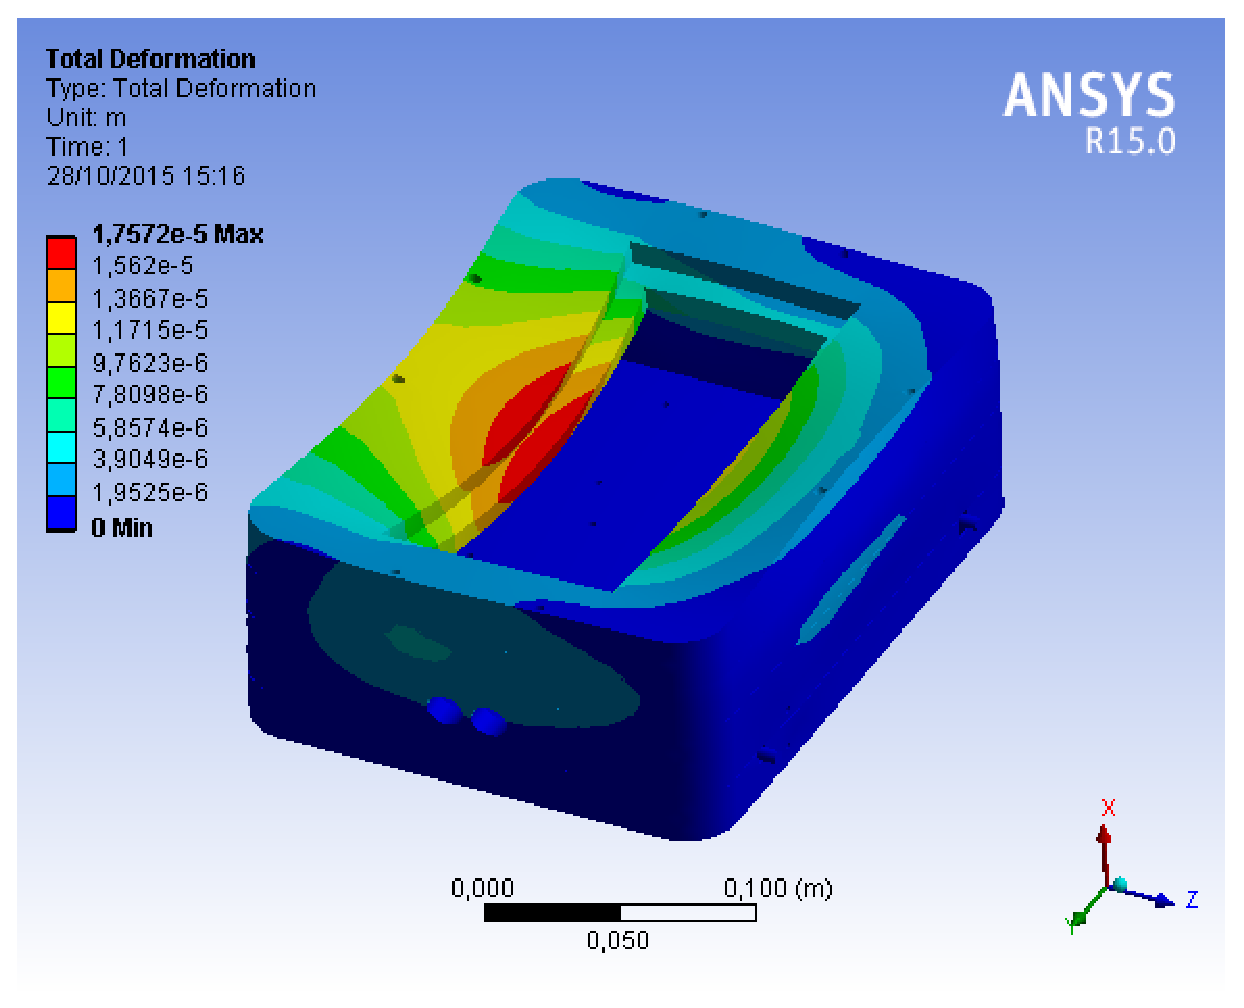
\includegraphics[width=0.8\textwidth]{figuras/deformacao_1000n.eps}
    \caption{}
    \label{fig:def1000}
\end{figure}

\begin{figure}[H]
    \centering
    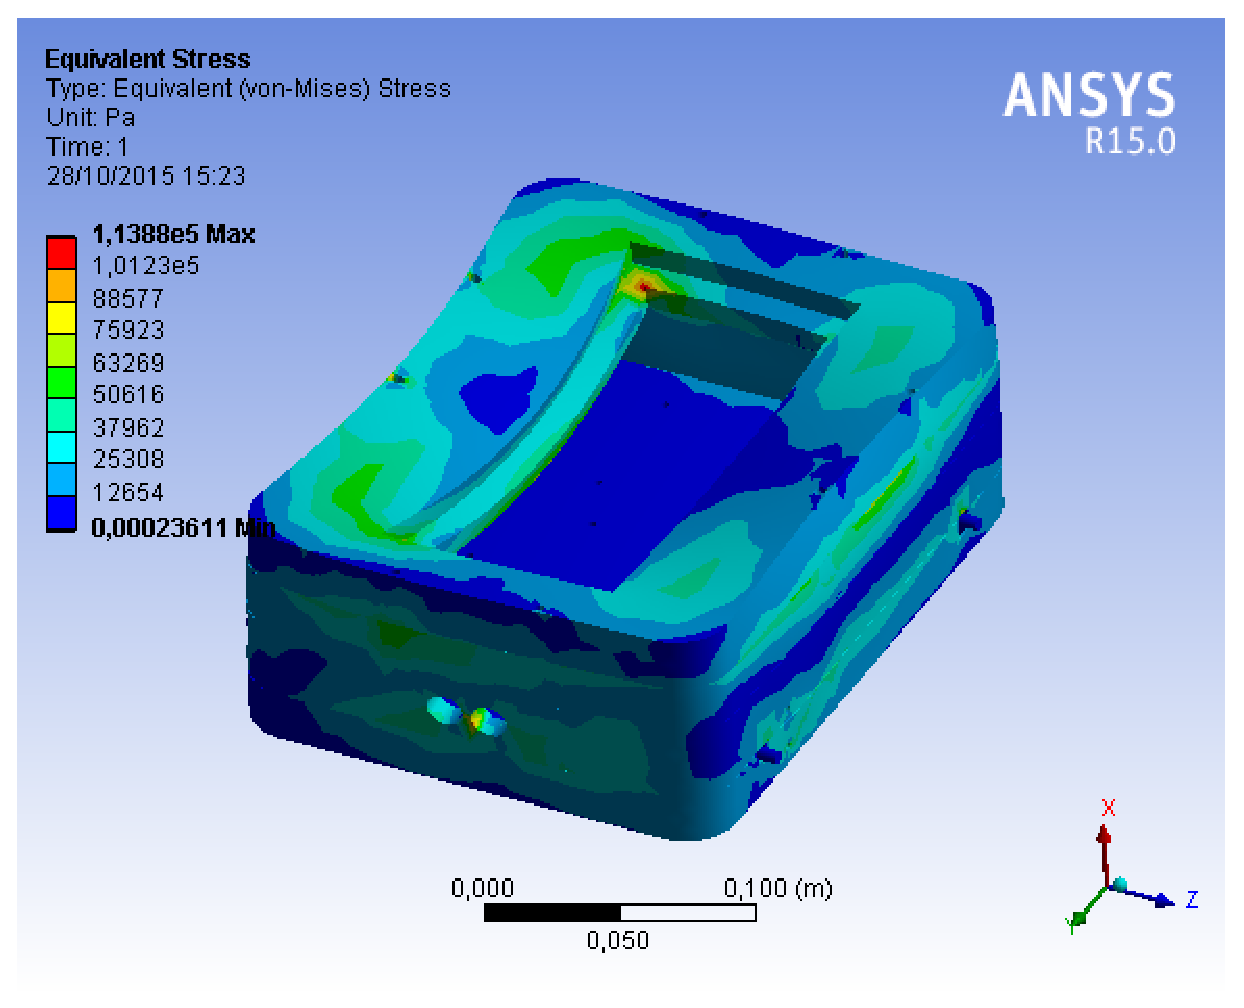
\includegraphics[width=0.8\textwidth]{figuras/vonmises_1000n.eps}
    \caption{}
    \label{fig:von1000}
\end{figure}

Nas ilustrações acima as condições de contorno são: Força de 1000 N (valor super estimado pela interação ser de impacto) na face superior,
força de 50 N na face lateral, a face inferior e os eixos fixos. Como podemos ver não ocorre nenhum deslocamento exagerado e a superfície
permanece a praticamente a mesma com o maior deslocamento sendo da ordem de 10e-5 m. Na análise do critério de Von Mises o maior valor
atingido é de 113,8 KPa o que é menor que os valores de ruptura dos materiais utilizados  na ordem de 10e3.
 
\textbf{Sobrepeso}: O caso estático fornece uma excelente resultado para o sobrepeso do carrinho, pois estamos analizando a estrutura com
o peso já em cima não o comportamento da estrutura ao impacto do peso. As condições de contorno usadas na análise foram: Força de 100 N
na parte superior do carrinho, eixos e parte inferior fixa (parte que não se move).
 
\textbf{Deformação}:

\begin{figure}[H]
    \centering
    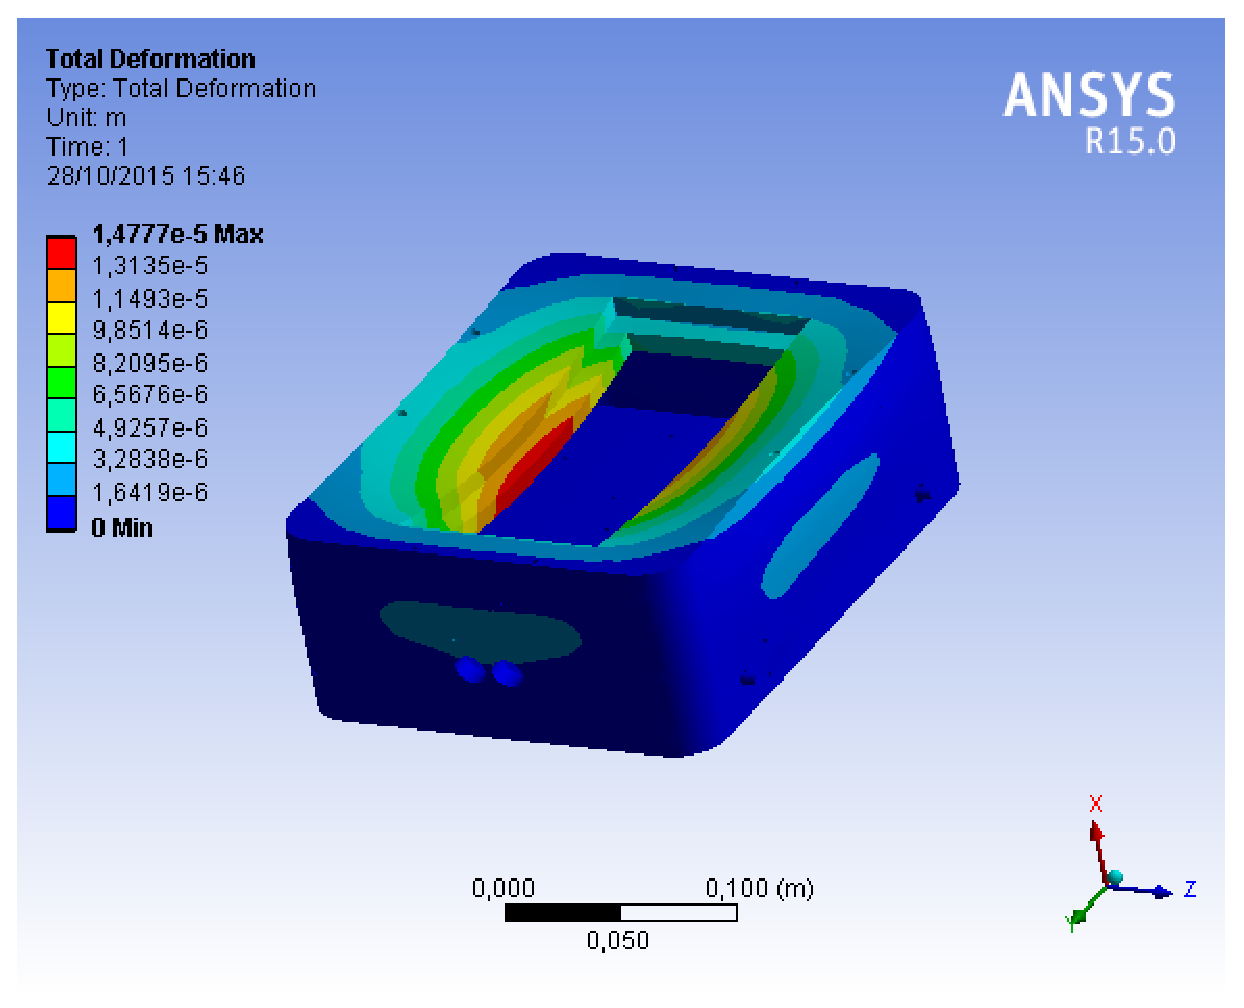
\includegraphics[width=0.8\textwidth]{figuras/deformacao_peso100n.eps}
    \caption{}
    \label{fig:def100}
\end{figure}

\begin{figure}[H]
    \centering
    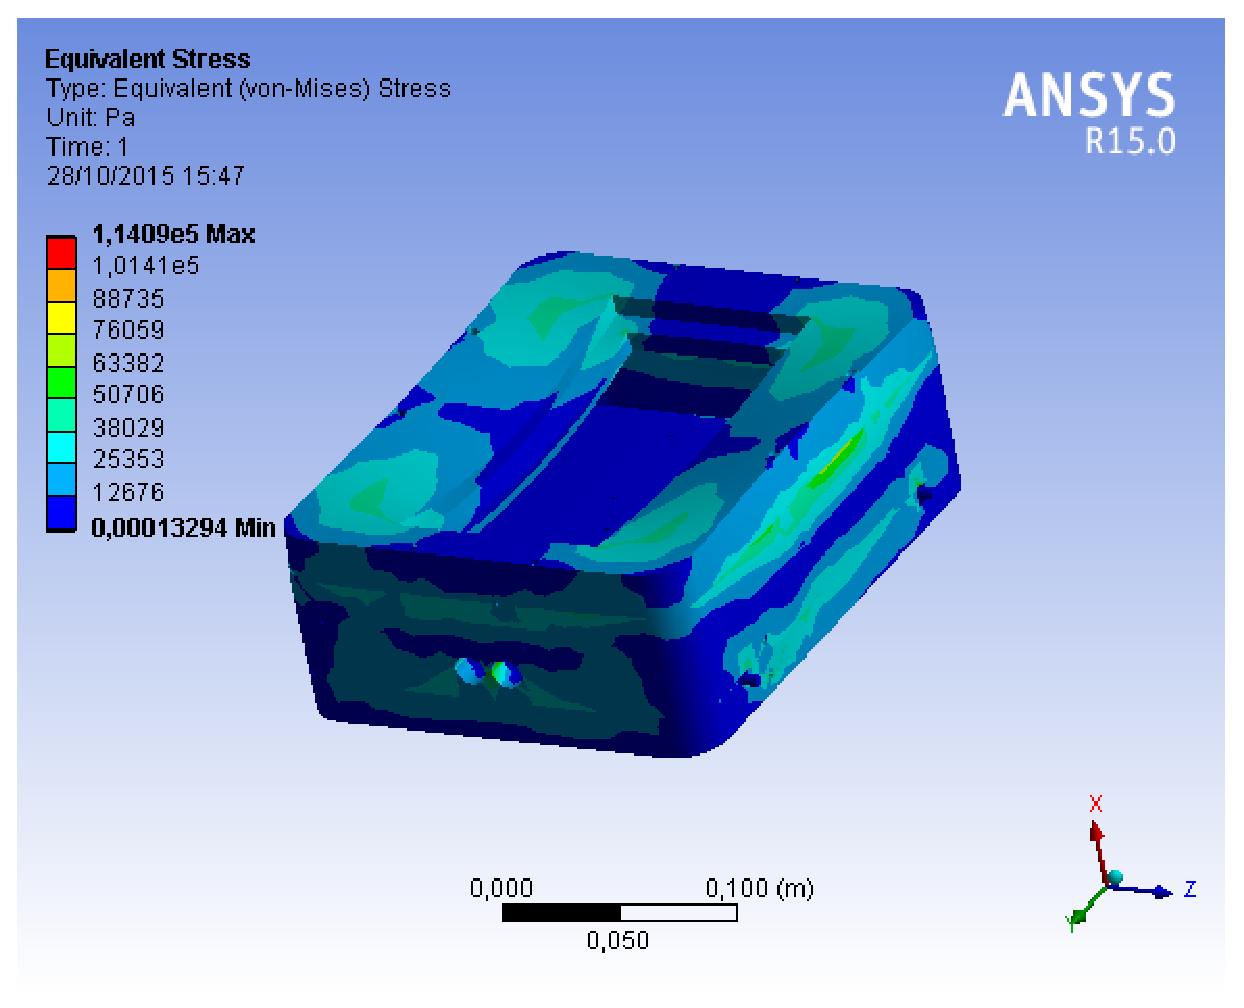
\includegraphics[width=0.8\textwidth]{figuras/vonmises_100n.eps}
    \caption{}
    \label{fig:von100}
\end{figure}

Como podemos ver o valor máximo da deformação é da ordem de 10e-5m o que significa que nessas condições não ocorre uma deformação expressiva no carrinho. Os valores da tensão de Von Mises não apresentam valores que possam oferecer um real risco a integridade do material pois apresentam valores da ordem de 10e3 menores que o valor da tensão de ruptura do material.
 
Choque com obstáculos: A velocidade do carrinho é relativamente baixa, em um impacto a magnitude das forças envolvidas são bem menores do que a magnitude das forças atuando na queda, como a simulação da queda validou a estrutura do carrinho estendemos os resultados para a análise de colisões e afirmamos que a estrutura desenvolvida está apta a colidir nas condições normais de operação do carrinho.
 
Como a estrutura desenvolvida não apresentou problemas em nenhum dos casos simulado, podemos afirmar que a estrutura cumpre os requisitos do projeto e portanto o seu uso é valido.

\subsection{Atuadores}

Os atuadores são os componentes que convertem a energia em potência mecânica, no caso em questão utilizaremos uma bateria para alimentação do alfa. Por meio de conversão eletromecânica a energia elétrica é convertida em potência mecânica e enviada para os elos, responsáveis pela movimentação do alfa.  Os atuadores utilizados em robôs de modo geral, são os atuadores eletromagnéticos, principalmente os que utilizam motores de corrente contínua e de passo. Os motores elétricos são interessantes no projeto de robôs, devido ao fato de que estes quando associado a sensores possibilitam tanto o controle de força quanto de posicionamento do robô, a facilidade na programação dos seus movimentos, visto que são controlados por sinais elétricos, até a utilização de controladores de movimentos (ROMANO \& DUTRA, 2002).

Os motores elétricos são divididos basicamente em: motores de corrente alternada (ca/ac) e motores de corrente continua (cc/dc). Os motores de corrente alternada são vantajosos devido a sua construção ser bastante simples, e a sua alimentação ocorrer diretamente da rede. No entanto nos projetos na área da robótica os motores de corrente contínua são os mais utilizados, devido a alimentação nestes tipos de projeto ocorrem na sua grande maioria a partir de bateria, as quais funcionam com corrente contínua, com isso a utilização de inversores não se faz necessária (BRAGA, 2006).


Além da alimentação dos motores de corrente contínua, outras vantagens em sua utilização, são devido: (BRAGA, 2006).
\begin{itemize}
	\item a velocidade do motor ser ajustada a partir de um potenciômetro, realizando a variação da tentão aplicada sobre o motor;
	\item o sentido de rotação do motor pode ser alterado a partir da alteração da polaridade da tensão aplicada ao motor;
	\item ao controle da aceleração e desaceleração do motor promovendo uma resposta no tempo ou para suavizar o funcionamento deste;
	\item a possibilidade de controle do torque a partir da variação da corrente aplicada no motor;
	\item a apresentarem uma resposta rápida, ou seja, quando submetidos a voltagens elevadas acelera rapidamente.
\end{itemize}

Os motores utilizado no alfa são motores dc, com caixa de redução 1:48, e eixo duplo, a escolha desse motor ocorreu devido aos fatores apresentados acima. Abaixo será apresentado uma tabela com as especificações do motor que será utilizado.

\begin{figure}[H]
    \centering
    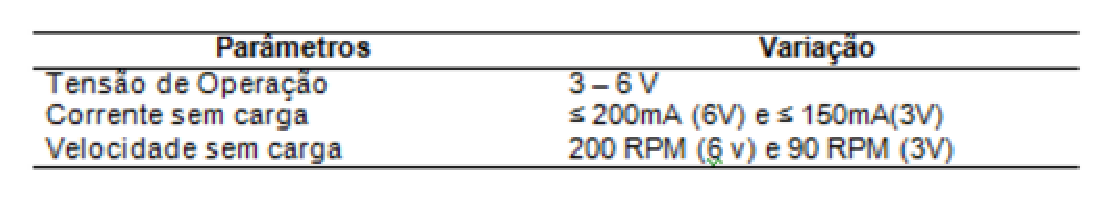
\includegraphics[width=0.5\textwidth]{figuras/tensao.eps}
    \caption{Especificações do motor utilizados no Alfa.}
    \label{fig:tensao}
\end{figure}

\begin{figure}[H]
    \centering
    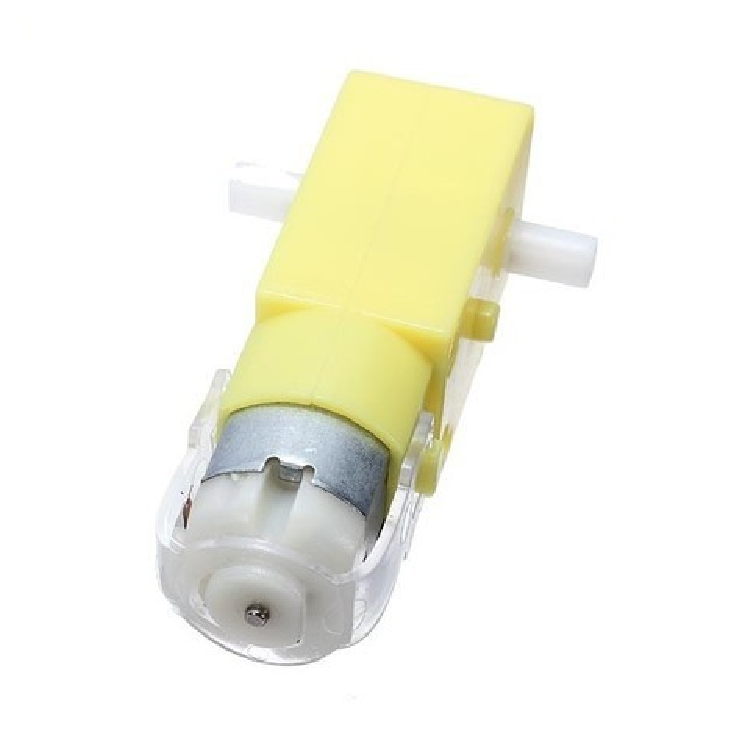
\includegraphics[width=0.8\textwidth]{figuras/motor.eps}
    \caption{Motor utilizado no robo Alfa. Fonte: Amazon S3 Web Services}
    \label{fig:motor}
\end{figure}

\subsection{Alimentação}

A alimentação dos componentes será feita por intermédio da placa Raspberry pi, o levantamento das necessidades energéticas delimitou que a placa necessita de uma tensão constante em 5 volts, recebendo 2 ampères de corrente.  Assim surgiram duas opções de alimentação: Pilhas ou Baterias.

As pilhas podem ser divididas em recarregáveis e não recarregáveis. As pilhas recarregáveis apesar de mais caras, possuem a vantagem de serem usadas em centenas de ciclos de carga e recarga. As de uso único tornam o projeto mais barato, entretanto o custo de troca de pilhas reaparece várias vezes para o consumidor. Independentemente do tipo de pilha utilizada, as pilhas comerciais apresentam valores de tensão e corrente muito abaixo do necessário, sendo necessário colocar várias em série para elevar a tensão e várias em paralelo, para elevar a corrente de alimentação. Isso acaba tornando o uso de pilhas nada prático.

Além de que a tensão de pilhas cai de acordo com a capacidade é utilizada, fazendo com que a placa desligasse antes da pilha estar totalmente carregada pelo fato da tensão não estar adequada, a figura abaixo ilustra (para uma pilha AA “heavy duty”).

\begin{figure}[H]
    \centering
    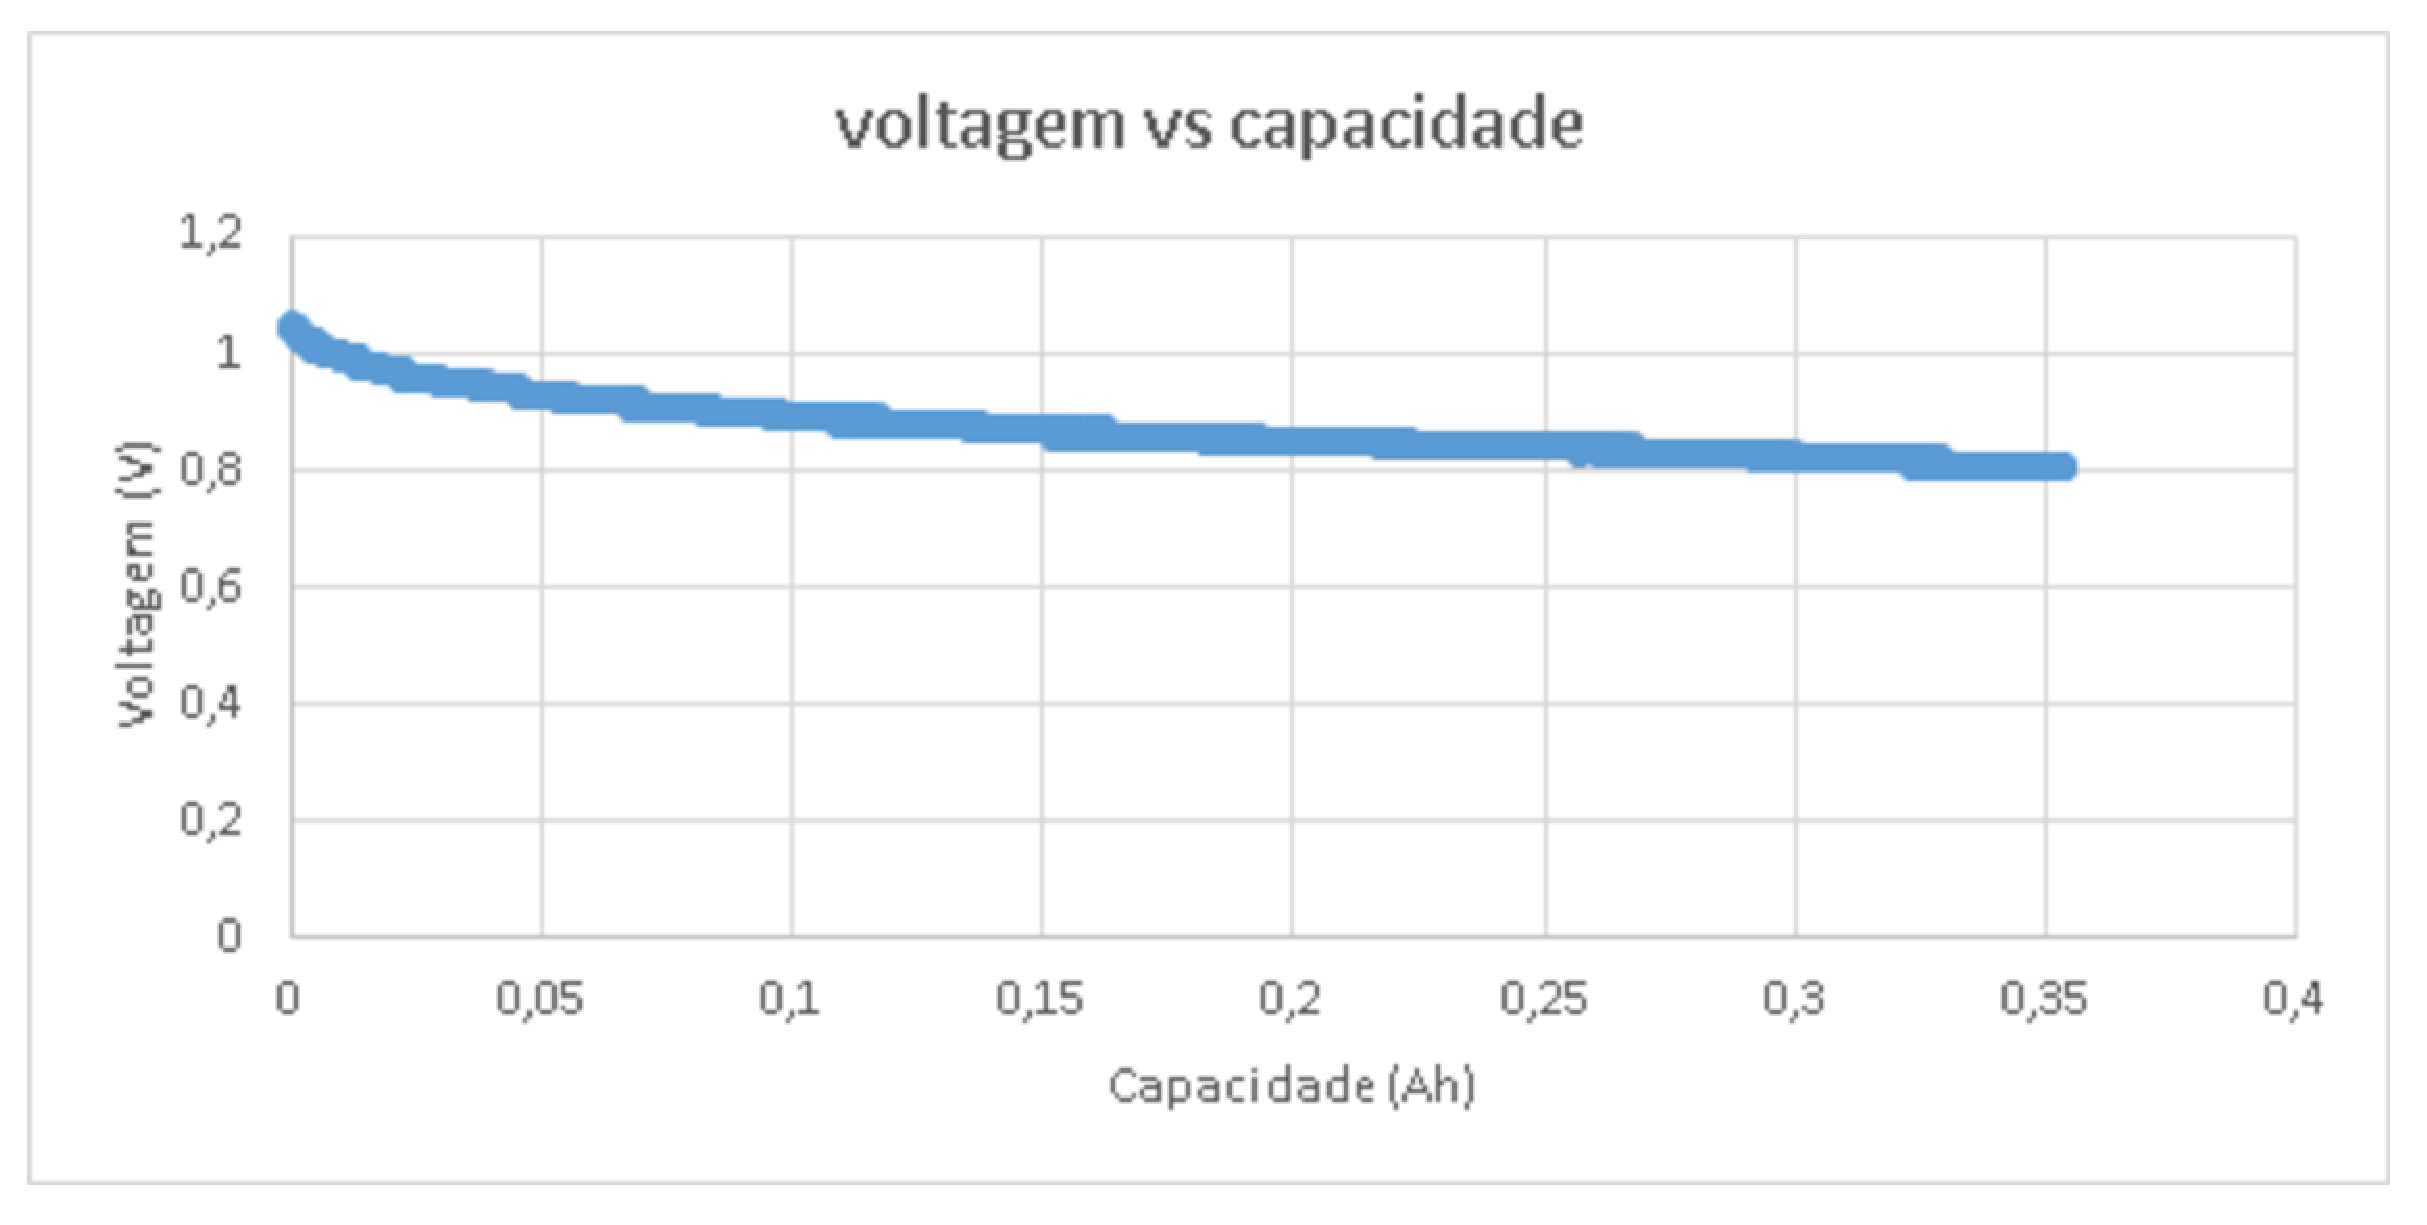
\includegraphics[width=0.8\textwidth]{figuras/volt_vs_cap.eps}
    \caption{curva de tensão vs capacidade de uma pilha AA}
    \label{fig:volts}
\end{figure}

As baterias encontradas no mercado podem ser de vários tipos, as mais comuns são as de Ion-Lítio, a maior vantagem delas é o seu fator energético em função do peso ser alto, elas costumam ser bem mais leves que outras baterias recarregáveis de mesmo tamanho (geralmente 150 watt-hora para cada quilo de bateria), além de serem bem mais baratas e seguras que outras baterias, como as de chumbo-ácido.

A bateria escolhida é a KMASHI MP816, por apresentar uma capacidade nominal de 10 Ah, atendendo ao projeto. Sua recarga é rápida e sua descarga pode ser controlada de acordo com a necessidade do projeto.  Para verificar se a carga real era próxima da nominal, um teste de carga foi realizado. O peso da bateria é de 280 gramas.

Ao se manter uma tensão constante de 5V e 2A (totalizando 10W de potência nominal para recarga) a bateria necessitou de em média 3 horas para atingir uma carga satisfatória (90\% da carga), em uma alimentação forçada de 4 horas, o nível de carga subiu pouco (em torno de 5\%) comparado às 3 horas iniciais. Logo o sistema possui um tempo de recarga para valores satisfatórios de 3 horas quando se utiliza uma fonte D.C. de 10 watts de potência. Para a descarga, o sistema apresenta um valor um pouco inferior. 2 horas e 50 minutos de autonomia em média, considerando que a carga será constante de 10,5 watts.

\subsection{Giro e Curvas}

Quando for enviado o sinal para que o carrinho gire para a direita e para a esquerda, um dos motores será desligado assim com a força do único motor ligado as duas rodas frontais acompanham a roda que está sendo estimulada pelo motor e auxiliam para que o robô complete o giro, dessa forma obedecendo o comando, (o motor que será desligado dependerá do sentido que o robô irá se mover.
 
O princípio de usar esteiras neste carrinho é que este poderá passar por locais em que o piso não é plano, sendo assim para o bom funcionamento das mesmas o carrinho terá dois motores  para mover as esteiras da direita e da esquerda independentes. 

\section{Visão e Controle e Processamento}

Esta seção mostra os itens relacionados ao controle e processamento dos dados de comunicação do sistema. O sistema, em uma visão ampla,
é dividido em dois subsistemas:

\begin{itemize}
\item Inserido no \textbf{raspberry}, responsável por realizar a interpretação e execução do conjunto de instrução do programa;
\item Inserido no aparelho mobile, responsável pela construção dos programas contendo os conjuntos de instruções;
\end{itemize}

Segue um diagrama de sequência com a visão geral de como o robô Alfa irá funcionar e da comunicação entre os sistemas:

\begin{figure}[H]
    \centering
    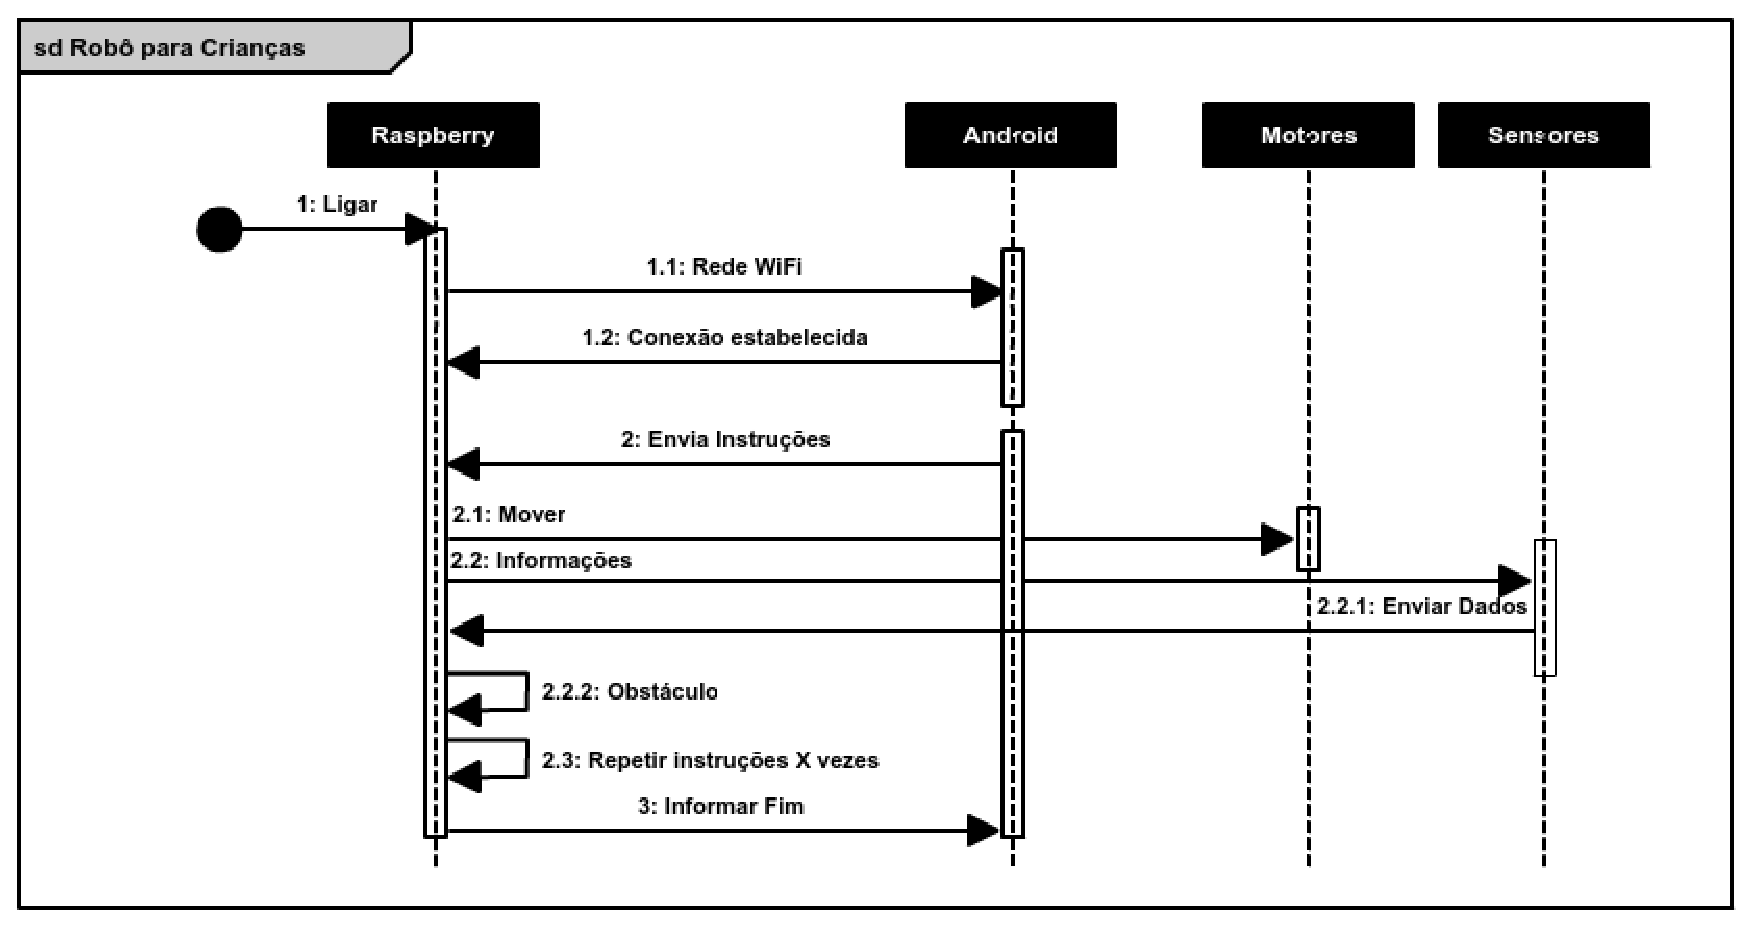
\includegraphics[width=0.8\textwidth]{figuras/diagrama_de_sequencia.eps}
    \caption{Diagrama de sequência - Visão geral dos sistemas}
    \label{fig:sequencia}
\end{figure}

\subsection{Configuração Wi-Fi}

Para o desenvolvimento da comunicação entre o robô educacional e o aplicativo em dispositivos móveis ANDROID escolheu-se a aplicação da tecnologia de comunicação wi-fi, de modo que é acoplado ao Raspberry Pi um dongle wi-fi (adaptador USB que adiciona funcionalidades à dispositivos, neste caso o adaptador wi-fi permite interação com este tipo de comunicação) para que se possa configurar propriamente o Raspberry Pi como um ponto de acesso de rede (Access Point ou Hotspot).

A tecnologia wi-fi foi escolhida por apresentar parâmetros que condizem com as necessidades do projeto (largura de banda – aproximadamente 22MHz – condizente com o requerido, alcance de aproximadamente 100 metros, menor latência, maior segurança, taxa de transmissão de bits – aproximadamente 600 Mbps - satisfatória para o projeto), outras tecnologias como por exemplo bluetooh, ZigBee e UWB não foram utilizadas por apresentarem características inferiores as desejadas para o projeto, inaplicabilidade ou por capacidade superior a requerida, respectivamente (IECON). Para a configuração do Raspberry Pi como Access Point instalou-se e configurou-se o protocolo de serviço DHCP (onde o mesmo utiliza um modelo cliente-servidor, gerenciando automaticamente os endereços de IP, gateway padrão, máscara de sub-rede e outros parâmetros da conexão dos dispositivos conectados ao access point), bem como instalou-se e configurou-se o Hostapd, que se trata de um programa no “user-space” que é executado em plano de fundo utilizado que realiza a autenticação de servidores e permite a criação de pontos de acesso (WIRELESS WIKI), neste caso, para o controle do robô. 

\begin{figure}[H]
    \centering
    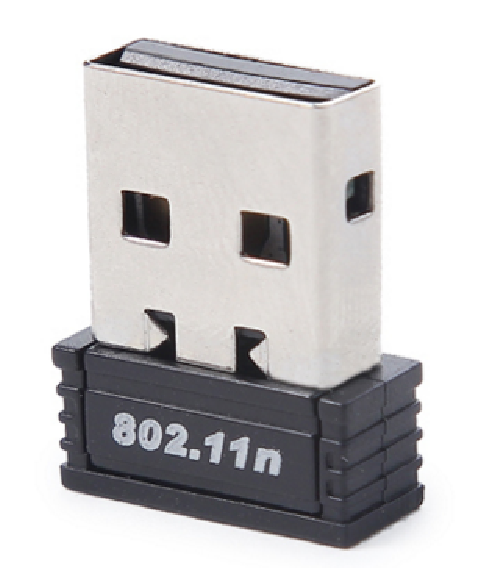
\includegraphics[width=0.4\textwidth]{figuras/adaptador_wifi.eps}
    \caption{ WiFi Dongle}
    \label{fig:catia01}
\end{figure}

\subsection{Alimentação}

Tendo em vista a necessidade de autonomia do robô um dos pontos fundamentais a serem desenvolvidos diz respeito a alimentação do Raspberry Pi. Para este projeto, inicialmente, decidiu-se alimentar o Raspberry Pi utilizando 6 (seis) pilhas do tipo AAA (que geram uma tensão igual a 9V) ou uma bateria 9V utilizando um circuito regulador de tensão implementando-se um CI7805 que fornece uma tensão fixa de saída igual a 5V e corrente máxima de 1.5 A o que é ideal para alimentação do Raspberry Pi (SPARKFUN).

Além disso utiliza-se dois capacitores, um capacitor em paralelo com a entrada do regulador de tensão e um outro capacitor em paralelo com a saída do regulador de tensão afim de evitar variações (ripples) no sinal de alimentação na entrada do regulador e na saída do regulador, respectivamente. É importante mencionar a implementação dos diodos para proteção contra correntes de polarização reversa. Para implantação deste circuito buscou-se a solução mais simples com melhor eficiência, atendendo os requisitos do projeto.

\begin{figure}[H]
    \centering
    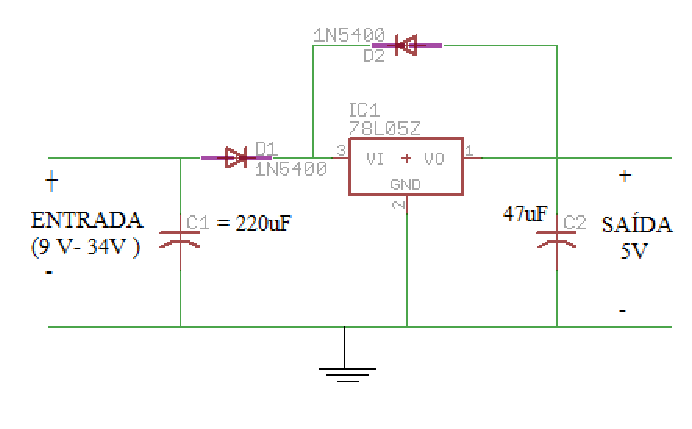
\includegraphics[width=0.8\textwidth]{figuras/esquematico_regulador.eps}
    \caption{Circuito regulador de tensão proposto para alimentação do Raspberry Pi}
    \label{fig:catia01}
\end{figure}

\subsection{Sensoriamento}

Em termos de interação com o ambiente na resposta do robô aos comandos fornecidos pela estrutura lógica de blocos do aplicativo, inicialmente realiza-se o sensoriamento utilizando-se um sensor de ultrassom na análise da distância do robô com relação aos objetos ao seu redor. Em princípio, implementa-se o sensoriamento de distância utilizando o modelo HC-RS04 que apresenta especificações de funcionamento (medição de distância de 2cm a 500cm, resolução de 0.3cm, frequência de 40kHz) e alimentação (5V DC) satisfatórias para a viabilização deste aspecto do projeto (MICROPIK).

Umas das terminações do sensor de ultrassom emite um pulso de duração de 10 microssegundos (pino trig é ativado), o sinal é refletido no objeto mais próximo e retorna para a segunda terminação onde aciona um de seus pinos (echo) sinalizando a chegada do sinal, o período de resposta (processamento) do sensor é igual a 50ms o que não leva a atrasos a serem considerados neste projeto. 

\begin{figure}[H]
    \centering
    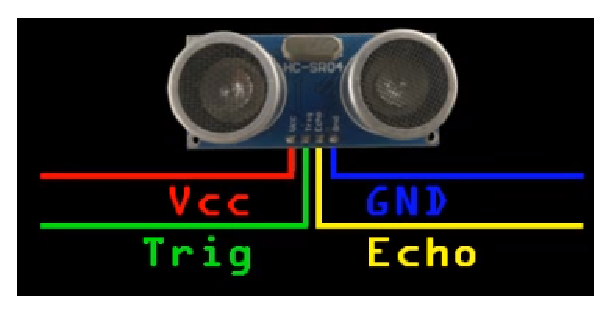
\includegraphics[width=0.5\textwidth]{figuras/pinos_ultrassom.eps}
    \caption{Sensor de Ultrassom HC-RS04 e respectivos pinos.}
    \label{fig:catia01}
\end{figure}

No que diz respeito a programação deste sensor é importante ressaltar que se deve considerar que o pulso emitido pelo sensor percorre duas vezes a distância entre o robô e o objeto, desta forma deve-se considerar a seguinte fórmula (levando-se em consideração a velocidade do som igual a 340m/s):

\begin{figure}[H]
    \centering
    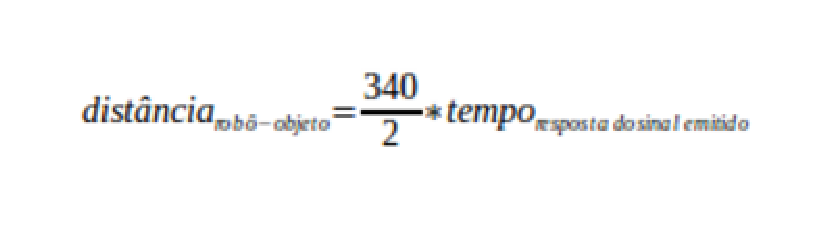
\includegraphics[width=0.4\textwidth]{figuras/distancia.eps}
    \caption{}
    \label{fig:catia01}
\end{figure}

Para implementação do sensor de ultrassom HC-RS04 deve-se considerar um divisor de tensão para o pino echo uma vez que este pino trabalha com uma tensão igual a 3.3V. Dessa maneira considerando um resistor  (que também atua como um resistor e pull-down), tem-se:

\begin{figure}[H]
    \centering
    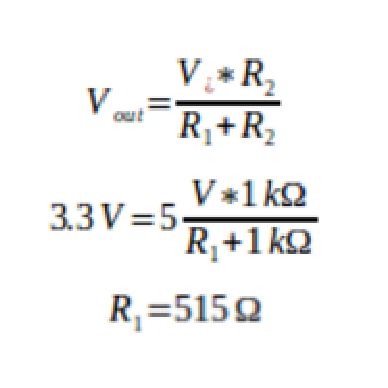
\includegraphics[width=0.3\textwidth]{figuras/vout.eps}
    \caption{}
    \label{fig:catia01}
\end{figure}

Dessa maneira utilizou-se um valor comercial disponível mais próximo igual a 680ohms. Pode-se observar o esquemático relativo a implementação do sensor de ultrassom a seguir:

\begin{figure}[H]
    \centering
    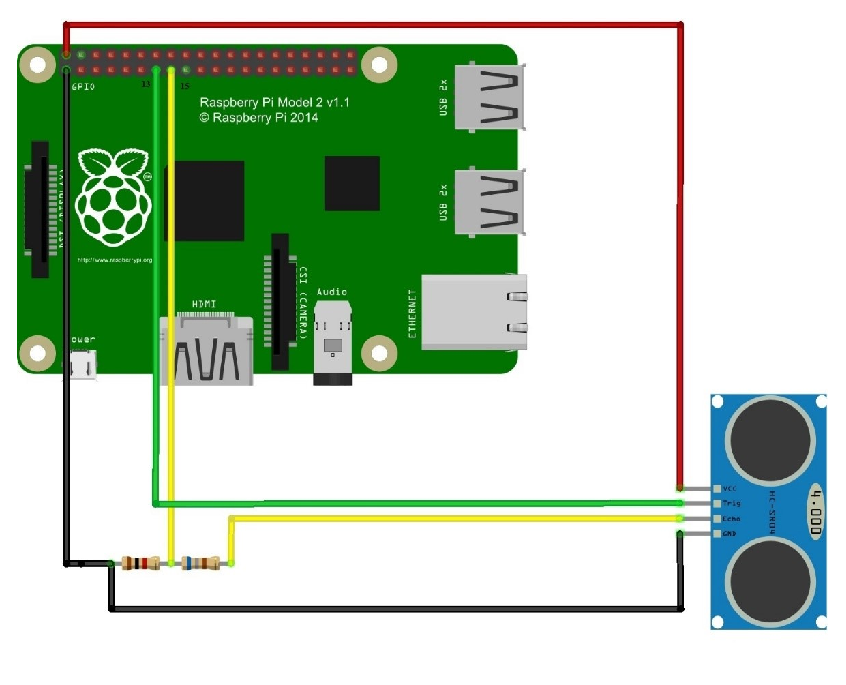
\includegraphics[width=0.8\textwidth]{figuras/esquematico_ultrassom.eps}
    \caption{Esquemático do circuito de implementação do sensor de ultrassom}
    \label{fig:catia01}
\end{figure}

O código referente a programação do sensor de distância ultrassom, em linguagem Python, está em Anexo A a este relatório.

\subsection{Comunicação Robô}

A comunicação entre o robô e o aplicativo mobile foi realizada através de uma comunicação do tipo Cliente/Servidor utilizando a API de Sockets em python, onde o servidor foi implementado no Raspberry PI, e o cliente foi configurado no aplicativo. Foi utilizado o protocolo TCP/IP na realização da comunicação, esse protocolo foi utilizado por ser atualmente o mais completo e aceito protocolo disponível, além de todos os sistemas operacionais modernos oferecerem suporte para o mesmo. Além disso o protocolo TCP/IP é do tipo stream, o que estabelece algumas características de transmissão, como confiabilidade, ordem, controle de fluxo e bidirecionalidade.

A seguir tem-se um diagrama ilustrando as funções utilizadas na implementação da comunicação cliente servidor utilizando o protocolo TCP/IP:

\begin{figure}[H]
    \centering
    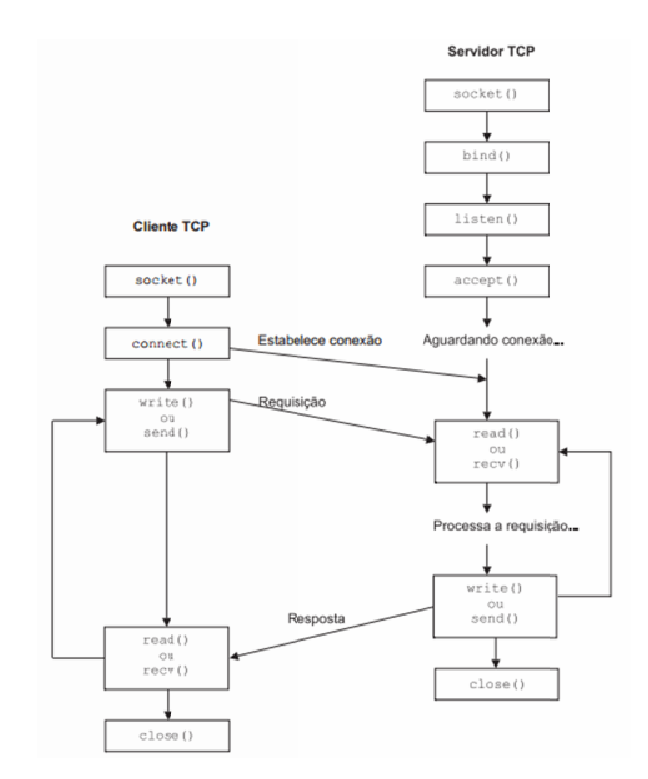
\includegraphics[width=0.8\textwidth]{figuras/diagrama_socket.eps}
    \caption{Diagrama de blocos do Sistema Cliente/Servidor utilizando TCP/IP}
    \label{fig:catia01}
\end{figure}

\subsection{Execução dos Blocos Lógicos}

As tarefas a serem executadas pelo robô são enviadas através de um arquivo do tipo JSON (Java Script Object Notation), onde o mesmo é recebido pelo servidor através da comunicação via sockets e interpretado a fim de executar as solicitações do usuário através da lógica de blocos. Para isso são passadas as chamadas das funções referentes a cada bloco lógico através do arquivo JSON, onde essas funções são lidas e interpretadas no Raspberry PI, com o intuito de ativar e controlar os motores do robô de acordo com as tarefas referentes a cada bloco lógico.

Os motores do robô são acionados e controlados utilizando 4 pinos GPIO do Raspberry PI e uma Ponte H. De modo que o Raspberry PI é responsável por enviar sinais PWM (configurados utilizando funções em python) para a Ponte H, referentes a velocidade e a direção que se deseja passar ao robô na execução de determinado bloco lógico. A Ponte H é responsável por inverter o sentido de rotação dos motores quando necessário, e também por sincronizar a inicialização e rotação dos mesmos.

\subsection{Ponte H}

A ponte H é um circuito designado para controlar o sentido e a velocidade dos motores DC do robô. Por ser um circuito do tipo chopper E, o mesmo circuito converte corrente contínua fixa em uma tensão de corrente contínua variável. Dessa forma, pode-se determinar o sentido da corrente e a polaridade da tensão. A ponte H é feita de componentes como Switches, Relays e Mosfets.

A figura abaixo mostra uma ponte H módulo L298N que foi utilizada no projeto. Este dispositivo foi utilizado considerando sua versatilidade e simplicidade de implementação, além de sua funcionalidade, como o controle de vários motores simultaneamente. Uma outra vantagem é o fato do L298N poder controlar as altas correntes dos motores, ela literalmente faz uma ‘ponte’ entre as correntes baixas do circuito lógico do Raspberry PI e dos motores DC utilizados para movimentar as rodas. As especificações do módulo L298N encontra-se abaixo:

I.	Chip: L298N
II.	Tensão Lógica: 5V
III.	Corrente Lógica: 0 mA - 36 mA
IV.	Temperatura de funcionamento: -20 C a +135 C
V.	Drive Voltage: 5V-35V
VI.	Drive current: 2A (MAX para uma ponte H)
VII.	Máxima Potência: 25W
VIII.	Dimensão: 43x43x27mm

\begin{figure}[H]
    \centering
    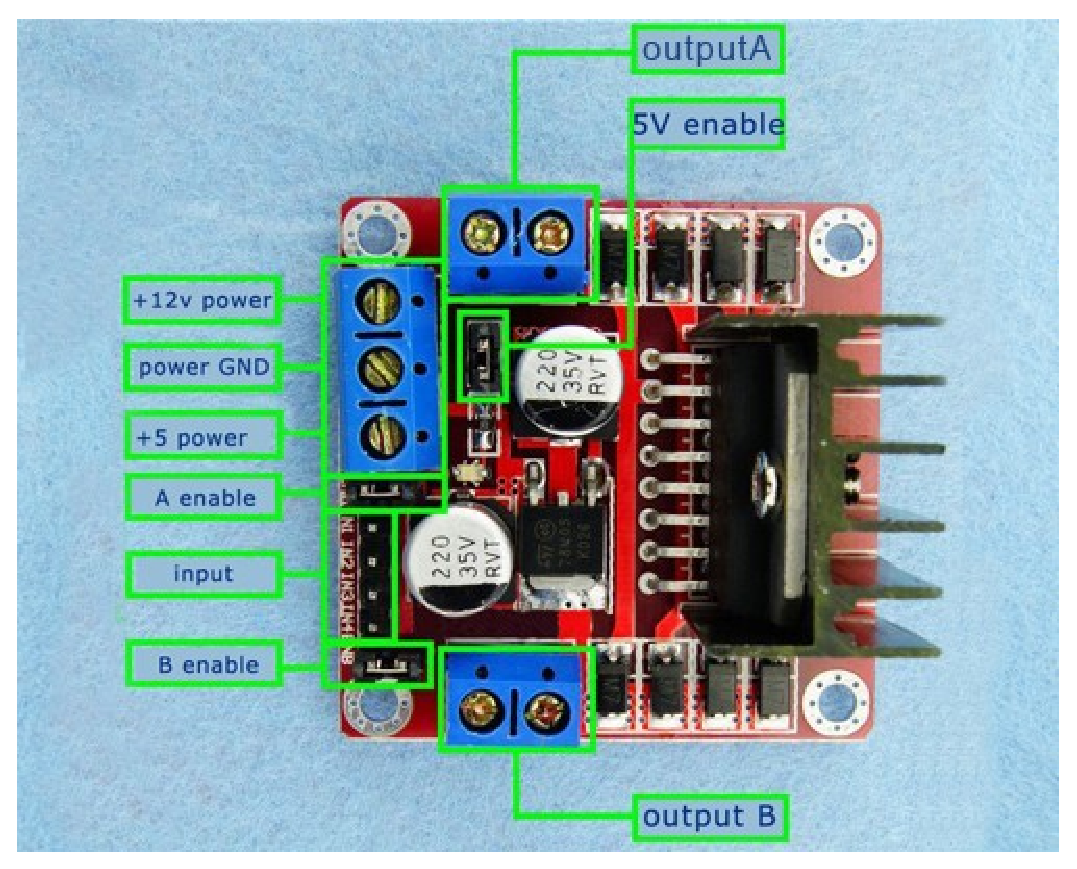
\includegraphics[width=0.8\textwidth]{figuras/ponteH.eps}
    \caption{Ponte H L298N e seus terminais. Fonte: Proesi - Componentes Eletrônicos}
    \label{fig:catia01}
\end{figure}

A conexão com o Raspberry Pi e os motores pode ser demonstrado pela figura Y. O terra do L298N é comum com o Raspberry, todavia necessita de uma alimentação externa, no caso 9V. Escolhe-se quatro pinos para serem ligados da ponte H ao Raspberry Pi, os mesmo pinos são definidos como saída no código, a figura Y ilustra a conexão de apenas dois pinos que saem da ponte H e fazem a conexão no Raspberry Pi. Controla-se as velocidades dos motores definindo a frequência do PWM e através do duty cycle é definido a porcentagem do tempo total que os motores estão na posição de trabalho. Utilizando a tabela X como referência, é possível definir o sentido dos motores e sua ação colocando os pinos em HIGH ou LOW  dependendo da fonte da alimentação. 

\begin{figure}[H]
    \centering
    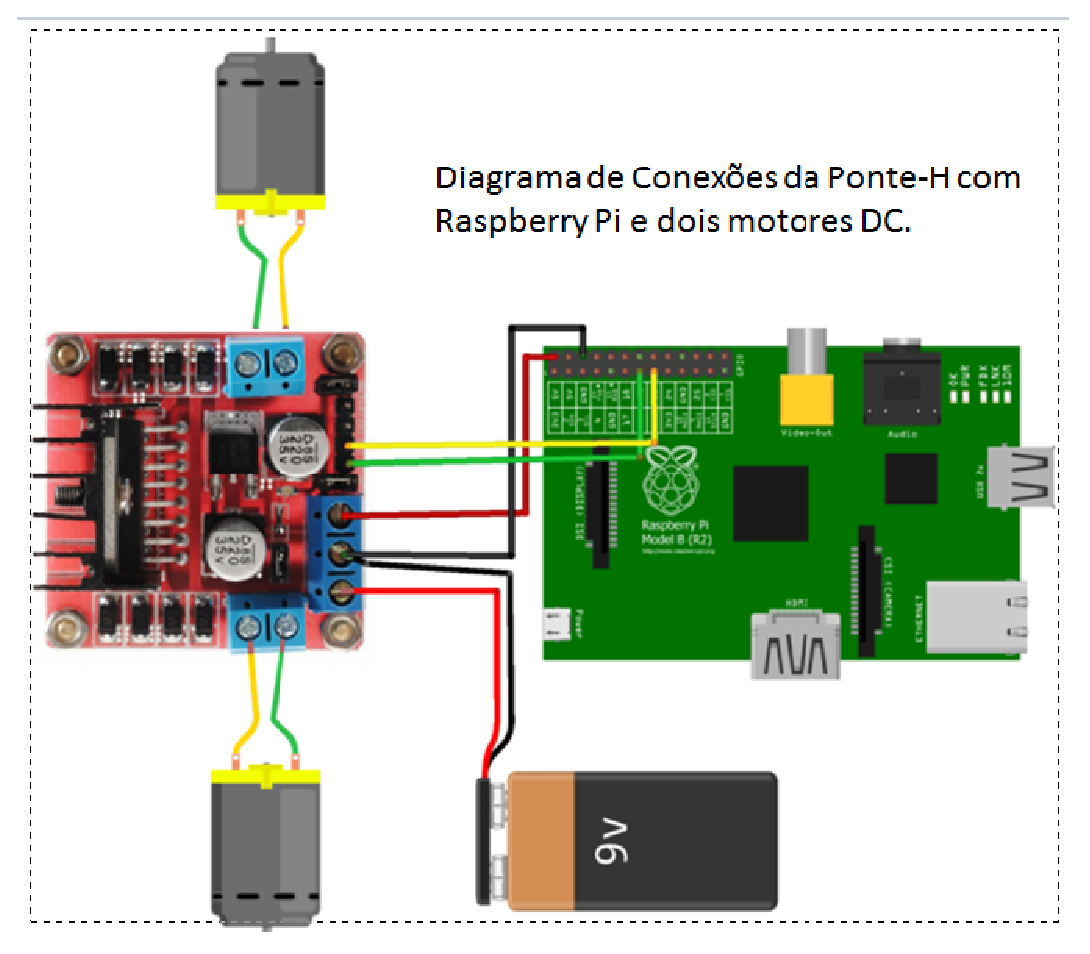
\includegraphics[width=0.8\textwidth]{figuras/esquematico_componentes.eps}
    \caption{Diagrama de conexões da Ponte H com periféricos.}
    \label{fig:catia01}
\end{figure}

\begin{figure}[H]
    \centering
    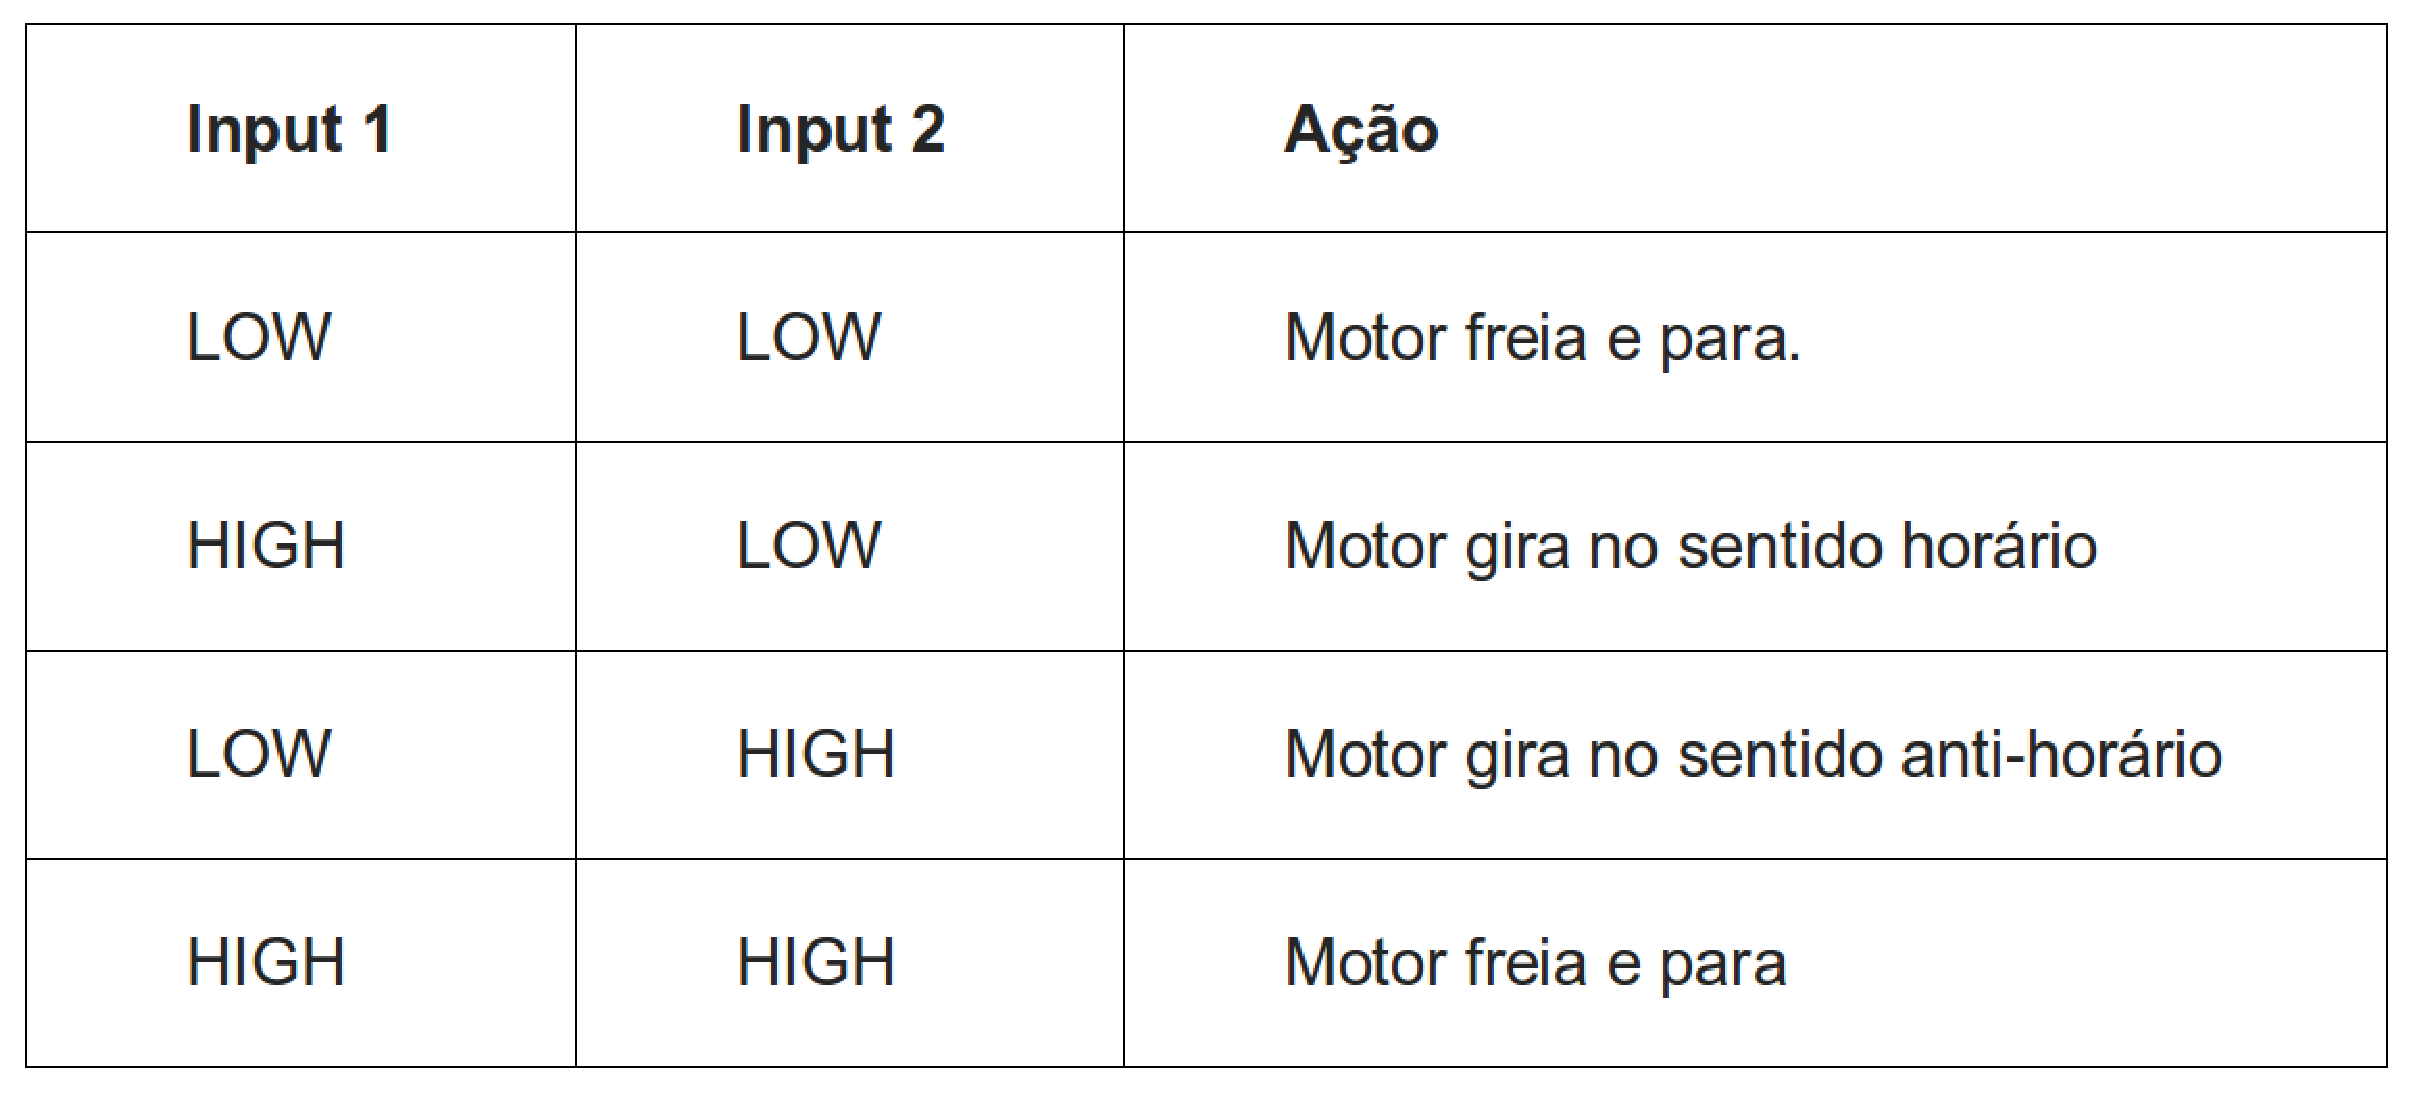
\includegraphics[width=0.8\textwidth]{figuras/tabela_ponte_H_2.eps}
    \caption{Tabela verdade utilizada no módulo Ponte H - Motor}
    \label{fig:catia01}
\end{figure}

\subsection{Aplicativo}
O aplicativo de controle do robô será implementada para o sistema operacional Android usando a linguagem de programação Java. A versão mínima do SDK será a 8 e a versão alvo será a 23. Por tanto as versões do SO suportadas serão da 2.2 (Froyo) até a 6.0 (Marshmallow).

Os métodos que merecem destaque são MyTouchListener() e a função de criação e envio das instruções:
\begin{itemize}
\item MyTouchListener(): responsável pelo monitoramento dos toques na tela do usuário. Implementada a partir da interface View.OnTouchListener
\item Função de criação e envio das instruções: após o usuário ordenar as instruções para o robô, essa função irá criar um arquivo JSON e enviar as instruções pela conexão WiFi via Socket.
\end{itemize}

As instruções estarão em arquivo JSON, criado no java a partir de JSONObject. Um exemplo de arquivo com as instruções é mostrado na figura abaixo:

\begin{figure}[H]
    \centering
    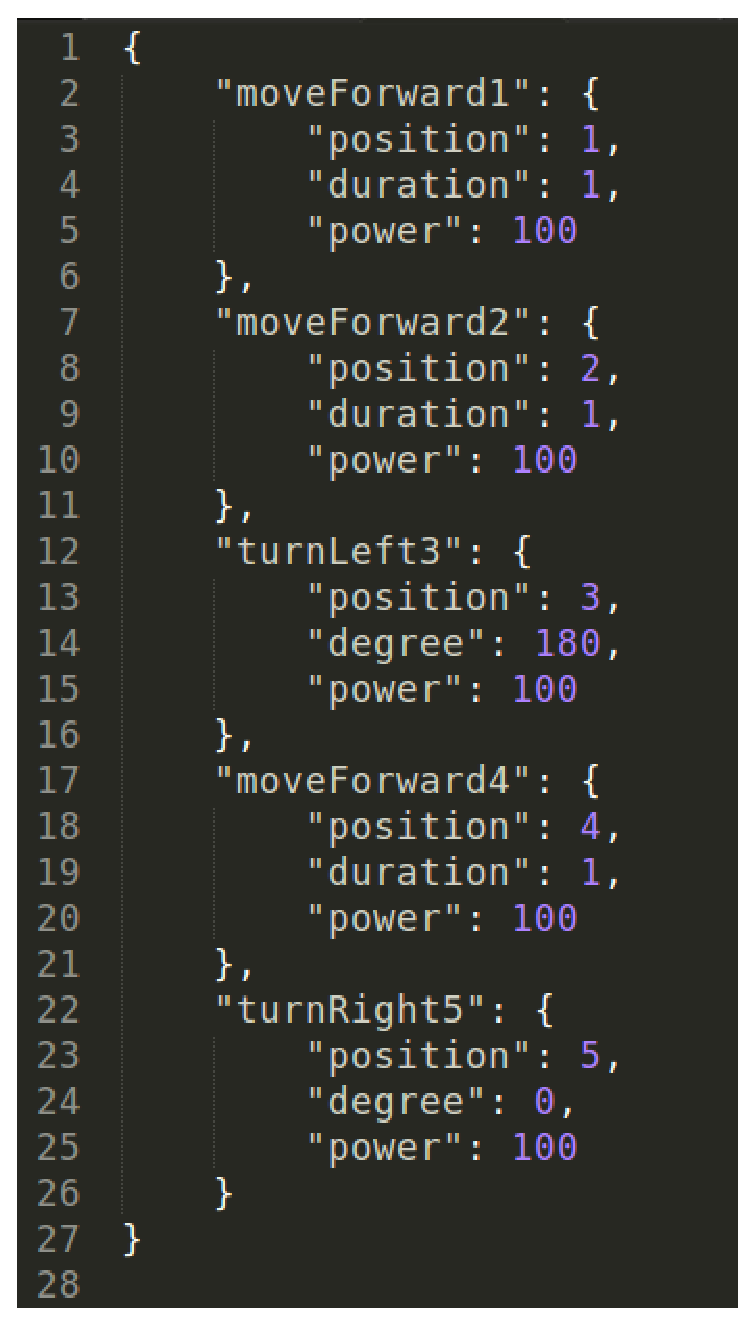
\includegraphics[width=0.4\textwidth]{figuras/exemplo_json.eps}
    \caption{Exemplo de Arquivo JSON}
    \label{fig:catia01}
\end{figure}

Os dados que esse arquivo irá enviar ao Raspberry Pi serão:
\begin{itemize}
	\item Comando/instrução: comando ou instrução para o robô, por exemplo vire a direita.
\end{itemize}

Dentro de cada comando/instrução os seguintes campos estão presentes:
\begin{itemize}
\item Position: posição em que determinada instrução está em todo o conjunto de blocos de instruções
\item Duration: no caso de “mover para frente”, será passada o tempo desse movimento. Cada tempo já é determinado: 1, 2, 5, 10. Cada uma dessas instruções será um bloco diferente na interface do aplicativo
\item Degree: são os graus com que o robô irá virar, caso seja necessário (ainda em avaliação).
\item Power: informação ainda em avaliação se será necessária para o robô, dado que todo o sistema de hardware e mecânico já está definido e não cabe ao aplicativo informar quanto de potência que o motor ou sensor deve ter.
\end{itemize}

Os outros blocos de instrução desejáveis na aplicação, a saber o de obstáculo para introdução do conceito das estruturas de condição e os círculos para introduzir os conceitos de laços de repetição ainda estão em desenvolvimento.